\documentclass{beamer}

\usepackage{beamerthemeCambridgeUS}
\usepackage{textpos}
\usepackage{ragged2e}
\usepackage{ulem}
\graphicspath{{G:/My Drive/FIGURAS/}}

\title[Geoforma: Componente Externo]{GEOMORFOLOGÍA}
\author[Edier Aristizabal]{Edier V. Aristizábal G.}
\institute{evaristizabalg@unal.edu.co}
\date{\tiny{Versión:\today}}

\addtobeamertemplate{headline}{}{%
	\begin{textblock*}{2mm}(.9\textwidth,0cm)
	\hfill\includegraphics[height=1cm]{un}  
	\end{textblock*}}

\begin{document}
%%%%%%%%%%%%%%%%%%%%%%%%%%%%%%%%%%%%%%%%%%%%%%%%%%%%%%%%%%%%%%%%%%%%%%%%%
\begin{frame}
\titlepage
\centering
   	\includegraphics[width=4cm]{unal} 
\end{frame}
%%%%%%%%%%%%%%%%%%%%%%%%%%%%%%%%%%%%%%%%%%%%%%%%%%%%%%%%%%%%%%%%%%%%%%%%%
\begin{frame}
\frametitle{Geoformas}
\scriptsize{Los atributos son características usadas para la descripción, identificación y clasificación de las geoformas. De acuerdo con Tricart (1965) y Van Zuidam (1985) se usan los siguientes tipos de atributos en un mapa geomorfológico detallado:\\
\vspace{5pt}
\textbf{Morfología}: el relieve general
\begin{itemize}
\item Morfografía para describir la geometría y aspectos de las geoformas
\item Morfométría para medir cuantitativamente las dimensiones de las geoformas
\end{itemize}
\textbf{Morfogenéticos}: para determinar el origen y la evolución de la geoformas
\begin{itemize}
\item Morfoestructura pasiva: la litología y estructuras relacionadas con proecesos denudacionales
\item Morfoestructura dinámica: la dinámica endógena
\item Morfodinámica: la dinámica exógena 
\end{itemize}
\textbf{Morfocronológicos}: para circunscribir el contexto temporal en que se originaron las geoformas
\begin{itemize}
\item Datación relativa
\item Datación absoluta
\end{itemize}
\textbf{Morfoarreglo}: el arreglo espacial y la interrelación de las diferentes geoformas y los procesos relacionados.
}\\
\vspace{5pt}
\tiny{Fuente: Zinck (1988) \& van Zuidam (1985)}
\end{frame}
%%%%%%%%%%%%%%%%%%%%%%%%%%%%%%%%%%%%%%%%%%%%%%%%%%%%%%%%%%%%%%%%%%%%%%%%%
\begin{frame}
\frametitle{Geoformas}
\small{Concepto genérico que designa todos los tipos de formas del relieve independiente de su origen, de su dimensión y de su nivel de abstracción.}
\begin{center}
\small{\textbf{Paisaje} (\emph{Landscape})$\rightarrow$agregado de \textbf{Geoformas} (\emph{Landform})$\rightarrow$forma+proceso}\\
   	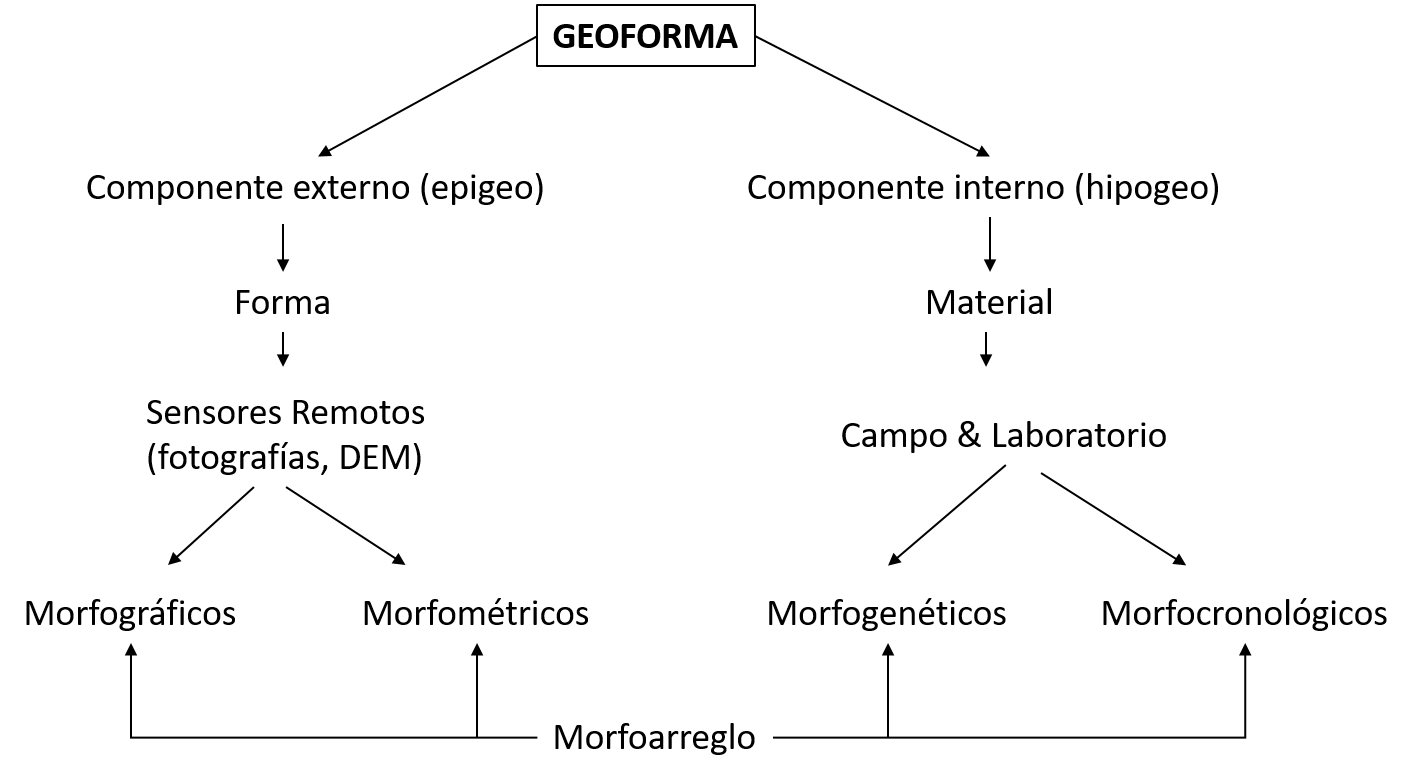
\includegraphics[scale=0.45]{geoforma1}
\end{center}
\tiny{Fuente: Zinck (1988)}
\end{frame}
%%%%%%%%%%%%%%%%%%%%%%%%%%%%%%%%%%%%%%%%%%%%%%%%%%%%%%%%%%%%%%%%%%%%%%%%%
\begin{frame}
\frametitle{Atributos}
\begin{center}
   	\includegraphics[scale=0.40]{atributos}
\end{center}
\tiny{Fuente: Zinck (1988)}
\end{frame}
%%%%%%%%%%%%%%%%%%%%%%%%%%%%%%%%%%%%%%%%%%%%%%%%%%%%%%%%%%%%%%%%%%%%%%%%%
 %#############################SLIDE
\begin{frame}
\frametitle{Sensores Remotos}
\scriptsize {Los \emph{Sensores Remotos} (teledetección) es el \textbf{arte, ciencia y tecnología} de observar un \textbf{objeto, escena o fenómeno} por técnicas basadas en instrumentos. El termino \emph{remoto} se refiere a la observación realizada a una distancia \textbf{sin contacto físico} con el objeto de interés. Se puede utilizar herramientas de detección y despliegue en tiempo real o una herramienta que registra la energía, la cual es emitida o reflejada desde el objeto o la escena en observación. La energía puede ser luz u otra forma de \textbf{radiaciones electromagnética}, campos de fuerza o energía acústica.}
\tiny{Fuente: ITC} 
  \begin{figure}
    \centering
    \includegraphics[height=.6\textheight]{definicion}
   \end{figure}
\end{frame}
%###############################%%%%%%%%%%%%%%%%%%%%%%
\begin{frame}
\frametitle{Espectro Electromagnético}
  \begin{figure}
    \centering
    \includegraphics[height=.34\textheight]{wave2}
    %\caption{This is the caption.}
  \end{figure}
\end{frame}
%################################SLIDE
\begin{frame}
\frametitle{Ventanas Atmosféricas}
\begin{center} 
\includegraphics[width=8cm]{ventanas}
\end{center}
\tiny{Credit: NASA's Imagine the Universe}
\end{frame}
%################################SLIDE
\begin{frame}
\frametitle{Radar vs Óptico}
\begin{center} 
\includegraphics[width=9cm]{radaroptico}
\end{center}
\tiny{Credit: NASA's Imagine the Universe}
\end{frame}
%################################SLIDE
\begin{frame}
\frametitle{Sensores}
  \begin{figure}
    \centering
    \includegraphics[height=.7\textheight]{activospasivos}
  \end{figure}
\end{frame}
%################################SLIDE
\begin{frame}
\frametitle{Sensores} 
 \begin{figure}
    \centering
    \includegraphics[height=.8\textheight]{sensores}
  \end{figure}
\end{frame}
%%%%%%%%%%%%%%%%%%%%%%%%%%%%%%%%%%%%%%%%%%%%%%%%%%%%%%%%%%%%%%
\begin{frame}
\frametitle{Detectores}
  \begin{columns}
		\begin{column}{.3\linewidth}
		 \includegraphics[width=4cm]{detector}
		\end{column}
		\begin{column}{.7\linewidth}
\includegraphics[width=8cm]{pixel}
		\end{column}
	\end{columns}
\end{frame}
%%%%%%%%%%%%%%%%%%%%%%%%%%%%%%%%%%%%%%%%%%%%%%%%%%%%%%%%%%%%%%
\begin{frame}
\frametitle{Estereoscopios}
  \begin{columns}
		\begin{column}{.3\linewidth}
		 \includegraphics[width=4cm]{estereoscopio}
		\end{column}
		\begin{column}{.3\linewidth}
\includegraphics[width=4cm]{estereoscopio2}
		\end{column}
		\begin{column}{.3\linewidth}
\includegraphics[width=4cm]{estereoscopio3}
		\end{column}
	\end{columns}
\end{frame}
%%%%%%%%%%%%%%%%%%%%%%%%%%%%%%%%%%%%%%%%%%%%%%%%%%%%%%%%%%%%%%%
%################################SLIDE
\begin{frame}
\frametitle{Sensores} 
 \begin{figure}
    \centering
    \includegraphics[height=.8\textheight]{rast1}
  \end{figure}
\end{frame}
%%%%%%%%%%%%%%%%%%%%%%%%%%%%%%%%%%%%%%%%%%%%%%%%%%%%%%%%%%%%%%
\begin{frame}
\frametitle{DEM} 
 \begin{figure}
    \centering
    \includegraphics[height=.8\textheight]{dtm5}
  \end{figure}
\end{frame}
%%%%%%%%%%%%%%%%%%%%%%%%%%%%%%%%%%%%%%%%%%%%%%%%%%%%%%%%%%%%%%
\begin{frame}
\frametitle{DEM} 
 \begin{figure}
    \centering
    \includegraphics[height=.8\textheight]{dtm6}
  \end{figure}
\end{frame}
%%%%%%%%%%%%%%%%%%%%%%%%%%%%%%%%%%%%%%%%%%%%%%%%%%%%%%%%%%%%%%
\begin{frame}
\frametitle{DEM} 
 \begin{figure}
    \centering
    \includegraphics[height=.8\textheight]{pixel3}
  \end{figure}
\end{frame}
%%%%%%%%%%%%%%%%%%%%%%%%%%%%%%%%%%%%%%%%%%%%%%%%%%%%%%%%%%%%%%
\begin{frame}
\frametitle{RADAR} 
 \begin{figure}
    \centering
    \includegraphics[height=.8\textheight]{shadow2}
  \end{figure}
\end{frame}
%%%%%%%%%%%%%%%%%%%%%%%%%%%%%%%%%%%%%%%%%%%%%%%%%%%%%%%%%%%%%%
\begin{frame}
\frametitle{Imágenes del óptico} 
 \begin{figure}
    \centering
    \includegraphics[height=.8\textheight]{imagen}
  \end{figure}
\end{frame}
%%%%%%%%%%%%%%%%%%%%%%%%%%%%%%%%%%%%%%%%%%%%%%%%%%%%%%%%%%%%%%
\begin{frame}
\frametitle{Imágenes del óptico} 
 \begin{figure}
    \centering
    \includegraphics[height=.8\textheight]{estuarios}
  \end{figure}
\end{frame}
%%%%%%%%%%%%%%%%%%%%%%%%%%%%%%%%%%%%%%%%%%%%%%%%%%%%%%%%%%%%%%
\begin{frame}
\frametitle{Imágenes del óptico} 
 \begin{figure}
    \centering
    \includegraphics[height=.8\textheight]{comparativo}
  \end{figure}
\end{frame}
%%%%%%%%%%%%%%%%%%%%%%%%%%%%%%%%%%%%%%%%%%%%%%%%%%%%%%%%%%%%%%
\begin{frame}
\frametitle{Imágenes disponibles} 
 \begin{figure}
    \centering
    \includegraphics[height=.8\textheight]{gee}
  \end{figure}
\end{frame}
%%%%%%%%%%%%%%%%%%%%%%%%%%%%%%%%%%%%%%%%%%%%%%%%%%%%%%%%%%%%%%
\begin{frame}
\frametitle{Imágenes disponibles} 
 \begin{figure}
    \centering
    \includegraphics[height=.75\textheight]{gee_landsat}
  \end{figure}
\end{frame}
%%%%%%%%%%%%%%%%%%%%%%%%%%%%%%%%%%%%%%%%%%%%%%%%%%%%%%%%%%%%%%
\begin{frame}
\frametitle{Imágenes disponibles} 
 \begin{figure}
    \centering
    \includegraphics[height=.7\textheight]{gee_dem}
  \end{figure}
\end{frame}
%%%%%%%%%%%%%%%%%%%%%%%%%%%%%%%%%%%%%%%%%%%%%%%%%%%%%%%%%%%%%%
\begin{frame}
\frametitle{Imágenes disponibles} 
 \begin{figure}
    \centering
    \includegraphics[height=.7\textheight]{alospalsar}
  \end{figure}
\end{frame}
%%%%%%%%%%%%%%%%%%%%%%%%%%%%%%%%%%%%%%%%%%%%%%%%%%%%%%%%%%%%%%
\begin{frame}
\frametitle{Imágenes disponibles} 
 \begin{figure}
    \centering
    \includegraphics[height=.7\textheight]{igac1}
  \end{figure}
\end{frame}
%%%%%%%%%%%%%%%%%%%%%%%%%%%%%%%%%%%%%%%%%%%%%%%%%%%%%%%%%%%%%%
\begin{frame}
\frametitle{Morfografía} 
 \begin{figure}
    \centering
    \includegraphics[height=.7\textheight]{formas}
  \end{figure}
\end{frame}
%%%%%%%%%%%%%%%%%%%%%%%%%%%%%%%%%%%%%%%%%%%%%%%%%%%%%%%%%%%%%%
\begin{frame}
\frametitle{Morfografía} 
 \begin{figure}
    \centering
    \includegraphics[height=.55\textheight]{regularidad}
  \end{figure}
\end{frame}
%%%%%%%%%%%%%%%%%%%%%%%%%%%%%%%%%%%%%%%%%%%%%%%%%%%%%%%%%%%%%%
\begin{frame}
\frametitle{Morfografía} 
 \begin{figure}
    \centering
    \includegraphics[height=.55\textheight]{relieve}
  \end{figure}
\end{frame}
%%%%%%%%%%%%%%%%%%%%%%%%%%%%%%%%%%%%%%%%%%%%%%%%%%%%%%%%%%%%%%
\begin{frame}
\frametitle{Morfografía} 
 \begin{figure}
    \centering
    \includegraphics[height=.55\textheight]{relieve1}
  \end{figure}
\end{frame}
%%%%%%%%%%%%%%%%%%%%%%%%%%%%%%%%%%%%%%%%%%%%%%%%%%%%%%%%%%%%%%
\begin{frame}
\frametitle{Morfografía} 
 \begin{figure}
    \centering
    \includegraphics[height=.55\textheight]{crestas}
  \end{figure}
\end{frame}
%%%%%%%%%%%%%%%%%%%%%%%%%%%%%%%%%%%%%%%%%%%%%%%%%%%%%%%%%%%%%%
\begin{frame}
\frametitle{Morfografía} 
 \begin{figure}
    \centering
    \includegraphics[height=.55\textheight]{longitud}
  \end{figure}
\end{frame}
%%%%%%%%%%%%%%%%%%%%%%%%%%%%%%%%%%%%%%%%%%%%%%%%%%%%%%%%%%%%%%
\begin{frame}
\frametitle{Geomorfometría}
\scriptsize{La medida y análisis de las características de geoformas que son aplicable a cualquier superficie continua. En general la Geomorfometría provee una base para la comparación cuantitativa de diferentes paisajes, y puede adaptar métodos de análisis de superficie por fuera de la geomorfología.} 
 \begin{figure}
    \centering
    \includegraphics[height=.7\textheight]{geomorfometria}
  \end{figure}
\end{frame}
%%%%%%%%%%%%%%%%%%%%%%%%%%%%%%%%%%%%%%%%%%%%%%%%%%%%%%%%%%%%%%
\begin{frame}
\frametitle{Geomorfometría}
\small{\textbf{Variables morfométricas}:\\
Una variable (atributo) morfométrica (topográfica) es un solo valor de una función bivariada que describe las propiedades de la superficie topográfica.\\
\vspace{10pt}
Existen 5 tipos principales de variables morfométricas:
\begin{itemize}
\item Variables locales
\item Variables no locales
\item Líneas estructurales
\item Variables solares
\item Variables combinadas
\end{itemize}
} 
\end{frame}
%%%%%%%%%%%%%%%%%%%%%%%%%%%%%%%%%%%%%%%%%%%%%%%%%%%%%%%%%%%%%%
\begin{frame}
\frametitle{Variables morfométricas locales}
\small{Es un solo valor de una función bivariado que describe la geometría de la superficie topográfica en la vecindad de un punto dado de la superficie.} 
 \begin{figure}
    \centering
    \includegraphics[height=.7\textheight]{morfolocales}
  \end{figure}
\end{frame}
%%%%%%%%%%%%%%%%%%%%%%%%%%%%%%%%%%%%%%%%%%%%%%%%%%%%%%%%%%%%%%
\begin{frame}
\frametitle{Variables morfométricas locales}
 \begin{figure}
    \centering
    \includegraphics[height=.7\textheight]{morfolocales1}
  \end{figure}
\end{frame}
%%%%%%%%%%%%%%%%%%%%%%%%%%%%%%%%%%%%%%%%%%%%%%%%%%%%%%%%%%%%%%
\begin{frame}
\frametitle{Variables morfométricas no locales}
 \begin{figure}
    \centering
    \includegraphics[height=.7\textheight]{morfonolocales}
  \end{figure}
\end{frame}
%%%%%%%%%%%%%%%%%%%%%%%%%%%%%%%%%%%%%%%%%%%%%%%%%%%%%%%%%%%%%%
\begin{frame}
\frametitle{Variables morfométricas solares y combinadas}
 \begin{figure}
    \centering
    \includegraphics[height=.7\textheight]{morfometricas}
  \end{figure}
\end{frame}
%%%%%%%%%%%%%%%%%%%%%%%%%%%%%%%%%%%%%%%%%%%%%%%%%%%%%%%%%%%%%%
\begin{frame}
\frametitle{Pendiente}
 \begin{figure}
    \centering
    \includegraphics[height=.6\textheight]{kernel1}
  \end{figure}
\end{frame}
%%%%%%%%%%%%%%%%%%%%%%%%%%%%%%%%%%%%%%%%%%%%%%%%%%%%%%%%%%%%%%
\begin{frame}
\frametitle{Pendiente}
 \begin{figure}
    \centering
    \includegraphics[height=.76\textheight]{pendiente}
  \end{figure}
\end{frame}
%%%%%%%%%%%%%%%%%%%%%%%%%%%%%%%%%%%%%%%%%%%%%%%%%%%%%%%%%%%%%%
\begin{frame}
\frametitle{Pendiente}
 \begin{figure}
    \centering
    \includegraphics[height=.55\textheight]{pendiente1}
    \includegraphics[height=.55\textheight]{pendiente2}
  \end{figure}
\end{frame}
%%%%%%%%%%%%%%%%%%%%%%%%%%%%%%%%%%%%%%%%%%%%%%%%%%%%%%%%%%%%%%
\begin{frame}
 \begin{figure}
    \centering
    \includegraphics[height=.85\textheight]{elbrus}
  \end{figure}
\end{frame}
%%%%%%%%%%%%%%%%%%%%%%%%%%%%%%%%%%%%%%%%%%%%%%%%%%%%%%%%%%%%%%
\begin{frame}
 \begin{figure}
    \centering
    \includegraphics[height=.85\textheight]{pendienteelbrus}
  \end{figure}
\end{frame}
%%%%%%%%%%%%%%%%%%%%%%%%%%%%%%%%%%%%%%%%%%%%%%%%%%%%%%%%%%%%%%
\begin{frame}
 \begin{figure}
    \centering
    \includegraphics[height=.85\textheight]{aspecto}
  \end{figure}
\end{frame}
%%%%%%%%%%%%%%%%%%%%%%%%%%%%%%%%%%%%%%%%%%%%%%%%%%%%%%%%%%%%%%
\begin{frame}
 \begin{figure}
    \centering
    \includegraphics[height=.85\textheight]{areaacumulada}
  \end{figure}
\end{frame}
%%%%%%%%%%%%%%%%%%%%%%%%%%%%%%%%%%%%%%%%%%%%%%%%%%%%%%%%%%%%%%
\begin{frame}
\frametitle{Curvatura}
 \begin{figure}
    \centering
    \includegraphics[height=.8\textheight]{curvatura}
  \end{figure}
\end{frame}
%%%%%%%%%%%%%%%%%%%%%%%%%%%%%%%%%%%%%%%%%%%%%%%%%%%%%%%%%%%%%%
\begin{frame}
\frametitle{Curvatura}
 \begin{figure}
    \centering
    \includegraphics[height=.8\textheight]{curvatura1}
  \end{figure}
\end{frame}
%%%%%%%%%%%%%%%%%%%%%%%%%%%%%%%%%%%%%%%%%%%%%%%%%%%%%%%%%%%%%%
\begin{frame}
\frametitle{Curvatura}
 \begin{figure}
    \centering
    \includegraphics[height=.8\textheight]{curvatura3}
  \end{figure}
\end{frame}
%%%%%%%%%%%%%%%%%%%%%%%%%%%%%%%%%%%%%%%%%%%%%%%%%%%%%%%%%%%%%%
\begin{frame}
\frametitle{Curvatura Horizontal}
 \begin{figure}
    \centering
    \includegraphics[height=.8\textheight]{curvaturah}
  \end{figure}
\end{frame}
%%%%%%%%%%%%%%%%%%%%%%%%%%%%%%%%%%%%%%%%%%%%%%%%%%%%%%%%%%%%%%
\begin{frame}
\frametitle{Curvatura Vertical}
 \begin{figure}
    \centering
    \includegraphics[height=.8\textheight]{curvaturav}
  \end{figure}
\end{frame}
%%%%%%%%%%%%%%%%%%%%%%%%%%%%%%%%%%%%%%%%%%%%%%%%%%%%%%%%%%%%%%
\begin{frame}
\frametitle{Curvatura}
 \begin{figure}
    \centering
    \includegraphics[height=.75\textheight]{curvatura2}
  \end{figure}
\tiny{Ayalew \& Yamagishi (2003) en la cuenca Blue Nile (Etiopía)}
\end{frame}
%%%%%%%%%%%%%%%%%%%%%%%%%%%%%%%%%%%%%%%%%%%%%%%%%%%%%%%%%%%%%%
\begin{frame}
\frametitle{Geomorfometría para mapas geomorfológicos}
 \begin{figure}
    \centering
    \includegraphics[height=.8\textheight]{shary}
  \end{figure}
\end{frame}
%%%%%%%%%%%%%%%%%%%%%%%%%%%%%%%%%%%%%%%%%%%%%%%%%%%%%%%%%%%%%%
\begin{frame}
\frametitle{Índice Topográfico de Humedad}
 \begin{figure}
    \centering
    \includegraphics[height=.8\textheight]{indicetopografico}
  \end{figure}
  \tiny{Fuente: Gallay (2013)}
\end{frame}
%%%%%%%%%%%%%%%%%%%%%%%%%%%%%%%%%%%%%%%%%%%%%%%%%%%%%%%%%%%%%%
\begin{frame}
\frametitle{Parámetros morfométricos}
 \begin{figure}
    \centering
    \includegraphics[height=.8\textheight]{parametros}
  \end{figure}
\end{frame}
%%%%%%%%%%%%%%%%%%%%%%%%%%%%%%%%%%%%%%%%%%%%%%%%%%%%%%%%%%%%%%
\begin{frame}
\frametitle{Parámetros morfométricos}
 \begin{figure}
    \centering
    \includegraphics[height=.7\textheight]{parametros1}
  \end{figure}
\end{frame}
%%%%%%%%%%%%%%%%%%%%%%%%%%%%%%%%%%%%%%%%%%%%%%%%%%%%%%%%%%%%%%
\begin{frame}
\frametitle{Procedimiento DEM corregido}
 \begin{figure}
    \centering
    \includegraphics[height=.7\textheight]{dem_fill_meto}
  \end{figure}
\end{frame}
%%%%%%%%%%%%%%%%%%%%%%%%%%%%%%%%%%%%%%%%%%%%%%%%%%%%%%%%%%%%%%
\begin{frame}
\frametitle{Dirección del flujo}
 \begin{figure}
    \centering
    \includegraphics[height=.55\textheight]{direccionflujo}
  \end{figure}
\end{frame}
%%%%%%%%%%%%%%%%%%%%%%%%%%%%%%%%%%%%%%%%%%%%%%%%%%%%%%%%%%%%%%
\begin{frame}
\frametitle{Dirección del flujo}
 \begin{figure}
    \centering
    \includegraphics[height=.8\textheight]{direccionflujo1}
  \end{figure}
\end{frame}
%%%%%%%%%%%%%%%%%%%%%%%%%%%%%%%%%%%%%%%%%%%%%%%%%%%%%%%%%%%%%%
\begin{frame}
\frametitle{Perfiles}
 \begin{figure}
    \centering
    \includegraphics[height=.75\textheight]{gee_perfiles}
  \end{figure}
\end{frame}
%%%%%%%%%%%%%%%%%%%%%%%%%%%%%%%%%%%%%%%%%%%%%%%%%%%%%%%%%%%%%%
\begin{frame}
\frametitle{Perfiles}
 \begin{figure}
    \centering
    \includegraphics[height=.75\textheight]{swathprofile}
  \end{figure}
\end{frame}
%%%%%%%%%%%%%%%%%%%%%%%%%%%%%%%%%%%%%%%%%%%%%%%%%%%%%%%%%%%%%%
\begin{frame}
\frametitle{Índices Morfométricos}
 \begin{figure}
    \centering
    \includegraphics[height=.75\textheight]{wilford}
  \end{figure}
\end{frame}
%%%%%%%%%%%%%%%%%%%%%%%%%%%%%%%%%%%%%%%%%%%%%%%%%%%%%%%%%%%%%%
\begin{frame}
\frametitle{Índices Morfométricos}
 \begin{figure}
    \centering
    \includegraphics[height=.75\textheight]{aristizabalarango}
  \end{figure}
\end{frame}
%%%%%%%%%%%%%%%%%%%%%%%%%%%%%%%%%%%%%%%%%%%%%%%%%%%%%%%%%%%%%%
\begin{frame}
\frametitle{Abánicos en el Valle de Aburrá}
 \begin{figure}
    \centering
    \includegraphics[height=.8\textheight]{demvdea}
  \end{figure}
\end{frame}
%%%%%%%%%%%%%%%%%%%%%%%%%%%%%%%%%%%%%%%%%%%%%%%%%%%%%%%%%%%%%%
\begin{frame}
\frametitle{Abánicos en el Valle de Aburrá}
 \begin{figure}
    \centering
    \includegraphics[height=.8\textheight]{areaabanico}
  \end{figure}
\end{frame}
%%%%%%%%%%%%%%%%%%%%%%%%%%%%%%%%%%%%%%%%%%%%%%%%%%%%%%%%%%%%%%
\begin{frame}
\frametitle{Perfiles longitudinales}
 \begin{figure}
    \centering
    \includegraphics[height=.6\textheight]{perfil4}
  \end{figure}
\end{frame}
%%%%%%%%%%%%%%%%%%%%%%%%%%%%%%%%%%%%%%%%%%%%%%%%%%%%%%%%%%%%%%
\begin{frame}
\frametitle{Perfiles longitudinales}
 \begin{figure}
    \centering
    \includegraphics[height=.8\textheight]{perfil5}
  \end{figure}
\end{frame}
%%%%%%%%%%%%%%%%%%%%%%%%%%%%%%%%%%%%%%%%%%%%%%%%%%%%%%%%%%%%%%
\begin{frame}
\frametitle{Perfiles longitudinales}
 \begin{figure}
    \centering
    \includegraphics[height=.8\textheight]{perfil6}
  \end{figure}
\end{frame}
%%%%%%%%%%%%%%%%%%%%%%%%%%%%%%%%%%%%%%%%%%%%%%%%%%%%%%%%%%%%%%
\begin{frame}
\frametitle{Curva hipsométrica}
 \begin{figure}
    \centering
    \includegraphics[height=.8\textheight]{hipsometrica3}
  \end{figure}
\end{frame}
%%%%%%%%%%%%%%%%%%%%%%%%%%%%%%%%%%%%%%%%%%%%%%%%%%%%%%%%%%%%%%
\begin{frame}
\frametitle{Correlación entre Índices Morfométricos}
 \begin{figure}
    \centering
    \includegraphics[height=.9\textheight]{aristizabalarango1}
  \end{figure}
\end{frame}
%%%%%%%%%%%%%%%%%%%%%%%%%%%%%%%%%%%%%%%%%%%%%%%%%%%%%%%%%%%%%%
\begin{frame}
\frametitle{Índices Morfométricos}
 \begin{figure}
    \centering
    \includegraphics[height=.75\textheight]{aristizabalarango2}
  \end{figure}
\end{frame}
%%%%%%%%%%%%%%%%%%%%%%%%%%%%%%%%%%%%%%%%%%%%%%%%%%%%%%%%%%%%%%
\begin{frame}
\frametitle{Índices Morfométricos}
 \begin{figure}
    \centering
    \includegraphics[height=.55\textheight]{aristizabalarango3}
  \end{figure}
\end{frame}
%%%%%%%%%%%%%%%%%%%%%%%%%%%%%%%%%%%%%%%%%%%%%%%%%%%%%%%%%%%%%%
\begin{frame}
\frametitle{Índices Morfométricos}
 \begin{figure}
    \centering
    \includegraphics[height=.75\textheight]{aristizabalarango4}
  \end{figure}
\end{frame}
%%%%%%%%%%%%%%%%%%%%%%%%%%%%%%%%%%%%%%%%%%%%%%%%%%%%%%%%%%%%%%
\begin{frame}
\frametitle{Índices Morfométricos}
 \begin{figure}
    \centering
    \includegraphics[height=.75\textheight]{aristizabalarango5}
  \end{figure}
\end{frame}
%%%%%%%%%%%%%%%%%%%%%%%%%%%%%%%%%%%%%%%%%%%%%%%%%%%%%%%%%%%%%%
\begin{frame}
\frametitle{Índices Morfométricos}
 \begin{figure}
    \centering
    \includegraphics[height=.4\textheight]{aristizabalarango6}
  \end{figure}
\end{frame}
%%%%%%%%%%%%%%%%%%%%%%%%%%%%%%%%%%%%%%%%%%%%%%%%%%%%%%%%%%%%%%

\end{document}